\section{Model\-Car\-Dyn  Class Reference}
\label{classModelCarDyn}\index{ModelCarDyn@{Model\-Car\-Dyn}}
The same model as {\bf Model2DRigid\-Dyncar} {\rm (p.\,\pageref{classModel2DRigidDyncar})}. 


{\tt \#include $<$modelcar.h$>$}

Inheritance diagram for Model\-Car\-Dyn::\begin{figure}[H]
\begin{center}
\leavevmode
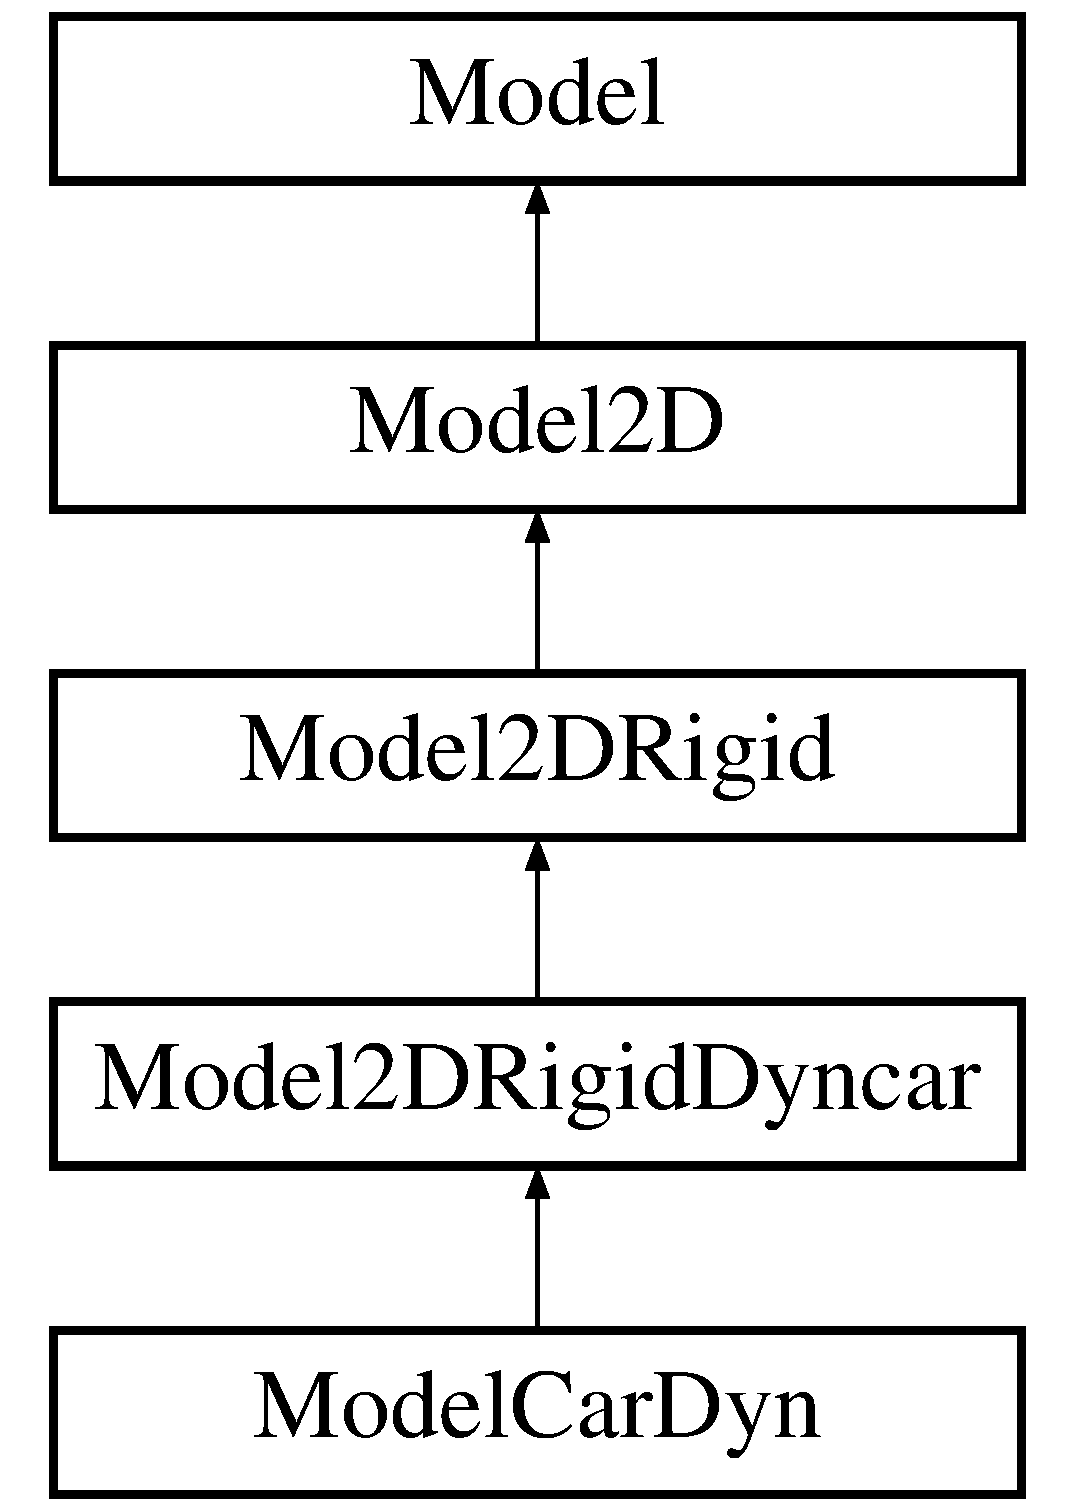
\includegraphics[height=5cm]{classModelCarDyn}
\end{center}
\end{figure}
\subsection*{Public Methods}
\begin{CompactItemize}
\item 
{\bf Model\-Car\-Dyn} (string path)
\item 
virtual {\bf $\sim$Model\-Car\-Dyn} ()
\item 
virtual {\bf MSLVector} {\bf State\-To\-Configuration} (const {\bf MSLVector} \&x)
\begin{CompactList}\small\item\em A method that converts a {\bf Model} {\rm (p.\,\pageref{classModel})} state in to a {\bf Geom} {\rm (p.\,\pageref{classGeom})} configuration.\item\end{CompactList}\item 
virtual double {\bf Metric} (const {\bf MSLVector} \&x1, const {\bf MSLVector} \&x2)
\begin{CompactList}\small\item\em A distance metric, which is Euclidean in the base class.\item\end{CompactList}\end{CompactItemize}


\subsection{Detailed Description}
The same model as {\bf Model2DRigid\-Dyncar} {\rm (p.\,\pageref{classModel2DRigidDyncar})}.



\subsection{Constructor \& Destructor Documentation}
\index{ModelCarDyn@{Model\-Car\-Dyn}!ModelCarDyn@{ModelCarDyn}}
\index{ModelCarDyn@{ModelCarDyn}!ModelCarDyn@{Model\-Car\-Dyn}}
\subsubsection{\setlength{\rightskip}{0pt plus 5cm}Model\-Car\-Dyn::Model\-Car\-Dyn (string {\em path} = \char`\"{}\char`\"{})}\label{classModelCarDyn_a0}


\index{ModelCarDyn@{Model\-Car\-Dyn}!~ModelCarDyn@{$\sim$ModelCarDyn}}
\index{~ModelCarDyn@{$\sim$ModelCarDyn}!ModelCarDyn@{Model\-Car\-Dyn}}
\subsubsection{\setlength{\rightskip}{0pt plus 5cm}Model\-Car\-Dyn::$\sim$Model\-Car\-Dyn ()\hspace{0.3cm}{\tt  [inline, virtual]}}\label{classModelCarDyn_a1}




\subsection{Member Function Documentation}
\index{ModelCarDyn@{Model\-Car\-Dyn}!Metric@{Metric}}
\index{Metric@{Metric}!ModelCarDyn@{Model\-Car\-Dyn}}
\subsubsection{\setlength{\rightskip}{0pt plus 5cm}double Model\-Car\-Dyn::Metric (const {\bf MSLVector} \& {\em x1}, const {\bf MSLVector} \& {\em x2})\hspace{0.3cm}{\tt  [virtual]}}\label{classModelCarDyn_a3}


A distance metric, which is Euclidean in the base class.



Reimplemented from {\bf Model2DRigid\-Dyncar} {\rm (p.\,\pageref{classModel2DRigidDyncar_a5})}.\index{ModelCarDyn@{Model\-Car\-Dyn}!StateToConfiguration@{StateToConfiguration}}
\index{StateToConfiguration@{StateToConfiguration}!ModelCarDyn@{Model\-Car\-Dyn}}
\subsubsection{\setlength{\rightskip}{0pt plus 5cm}{\bf MSLVector} Model\-Car\-Dyn::State\-To\-Configuration (const {\bf MSLVector} \& {\em x})\hspace{0.3cm}{\tt  [virtual]}}\label{classModelCarDyn_a2}


A method that converts a {\bf Model} {\rm (p.\,\pageref{classModel})} state in to a {\bf Geom} {\rm (p.\,\pageref{classGeom})} configuration.



Reimplemented from {\bf Model2DRigid\-Dyncar} {\rm (p.\,\pageref{classModel2DRigidDyncar_a3})}.

The documentation for this class was generated from the following files:\begin{CompactItemize}
\item 
{\bf modelcar.h}\item 
{\bf modelcar.C}\end{CompactItemize}
